%----------------------------------------------------------------------------------------
%	PACKAGES AND OTHER DOCUMENT CONFIGURATIONS
%----------------------------------------------------------------------------------------

\documentclass[11pt,fleqn]{book} % Default font size and left-justified equations

\usepackage[top=3cm,bottom=3cm,left=3.2cm,right=3.2cm,headsep=10pt,letterpaper]{geometry} % Page margins
\usepackage{CJKutf8}
\usepackage{xcolor} % Required for specifying colors by name
\definecolor{ocre}{RGB}{52,177,201} % Define the orange color used for highlighting throughout the book

% Font Settings
\usepackage{avant} % Use the Avantgarde font for headings
%\usepackage{times} % Use the Times font for headings
\usepackage{mathptmx} % Use the Adobe Times Roman as the default text font together with math symbols from the Sym­bol, Chancery and Com­puter Modern fonts
\usepackage{microtype} % Slightly tweak font spacing for aesthetics
\usepackage[utf8]{inputenc} % Required for including letters with accents
\usepackage[T1]{fontenc} % Use 8-bit encoding that has 256 glyphs
\usepackage{amsthm}
\usepackage{quiver} % to draw commutative diagrams

% Bibliography
\usepackage[style=alphabetic,sorting=nyt,sortcites=true,autopunct=true,babel=hyphen,hyperref=true,abbreviate=false,backref=true,backend=biber]{biblatex}
\addbibresource{bibliography.bib} % BibTeX bibliography file
\defbibheading{bibempty}{}

%----------------------------------------------------------------------------------------
%	VARIOUS REQUIRED PACKAGES
%----------------------------------------------------------------------------------------

\usepackage{titlesec} % Allows customization of titles

\usepackage{graphicx} % Required for including pictures
\graphicspath{{Pictures/}} % Specifies the directory where pictures are stored
% \graphicspath{{Plots/}}
\usepackage{lipsum} % Inserts dummy text

\usepackage{tikz} % Required for drawing custom shapes

\usepackage[english]{babel} % English language/hyphenation

\usepackage{enumitem} % Customize lists
\setlist{nolistsep} % Reduce spacing between bullet points and numbered lists

\usepackage{booktabs} % Required for nicer horizontal rules in tables

\usepackage{eso-pic} % Required for specifying an image background in the title page

%----------------------------------------------------------------------------------------
%	MAIN TABLE OF CONTENTS
%----------------------------------------------------------------------------------------

\usepackage{titletoc} % Required for manipulating the table of contents

\contentsmargin{0cm} % Removes the default margin
% Chapter text styling
\titlecontents{chapter}[1.25cm] % Indentation
{\addvspace{15pt}\large\sffamily\bfseries} % Spacing and font options for chapters
{\color{ocre!60}\contentslabel[\Large\thecontentslabel]{1.25cm}\color{ocre}} % Chapter number
{}  
{\color{ocre!60}\normalsize\sffamily\bfseries\;\titlerule*[.5pc]{.}\;\thecontentspage} % Page number
% Section text styling
\titlecontents{section}[1.25cm] % Indentation
{\addvspace{5pt}\sffamily\bfseries} % Spacing and font options for sections
{\contentslabel[\thecontentslabel]{1.25cm}} % Section number
{}
{\sffamily\hfill\color{black}\thecontentspage} % Page number
[]
% Subsection text styling
\titlecontents{subsection}[1.25cm] % Indentation
{\addvspace{1pt}\sffamily\small} % Spacing and font options for subsections
{\contentslabel[\thecontentslabel]{1.25cm}} % Subsection number
{}
{\sffamily\;\titlerule*[.5pc]{.}\;\thecontentspage} % Page number
[] 

%----------------------------------------------------------------------------------------
%	MINI TABLE OF CONTENTS IN CHAPTER HEADS
%----------------------------------------------------------------------------------------

% Section text styling
\titlecontents{lsection}[0em] % Indendating
{\footnotesize\sffamily} % Font settings
{}
{}
{}

% Subsection text styling
\titlecontents{lsubsection}[.5em] % Indentation
{\normalfont\footnotesize\sffamily} % Font settings
{}
{}
{}
 
%----------------------------------------------------------------------------------------
%	PAGE HEADERS
%----------------------------------------------------------------------------------------

\usepackage{fancyhdr} % Required for header and footer configuration

\pagestyle{fancy}
\renewcommand{\chaptermark}[1]{\markboth{\sffamily\normalsize\bfseries\chaptername\ \thechapter.\ #1}{}} % Chapter text font settings
\renewcommand{\sectionmark}[1]{\markright{\sffamily\normalsize\thesection\hspace{5pt}#1}{}} % Section text font settings
\fancyhf{} \fancyhead[LE,RO]{\sffamily\normalsize\thepage} % Font setting for the page number in the header
\fancyhead[LO]{\rightmark} % Print the nearest section name on the left side of odd pages
\fancyhead[RE]{\leftmark} % Print the current chapter name on the right side of even pages
\renewcommand{\headrulewidth}{0.5pt} % Width of the rule under the header
\addtolength{\headheight}{2.5pt} % Increase the spacing around the header slightly
\renewcommand{\footrulewidth}{0pt} % Removes the rule in the footer
\fancypagestyle{plain}{\fancyhead{}\renewcommand{\headrulewidth}{0pt}} % Style for when a plain pagestyle is specified

% Removes the header from odd empty pages at the end of chapters
\makeatletter
\renewcommand{\cleardoublepage}{
\clearpage\ifodd\c@page\else
\hbox{}
\vspace*{\fill}
\thispagestyle{empty}
\newpage
\fi}

%----------------------------------------------------------------------------------------
%	THEOREM STYLES
%----------------------------------------------------------------------------------------

\usepackage{amsmath,amsfonts,amssymb,amsthm} % For math equations, theorems, symbols, etc

\newcommand{\intoo}[2]{\mathopen{]}#1\,;#2\mathclose{[}}
\newcommand{\ud}{\mathop{\mathrm{{}d}}\mathopen{}}
\newcommand{\intff}[2]{\mathopen{[}#1\,;#2\mathclose{]}}
\newtheorem{notation}{Notation}[chapter]

%%%%%%%%%%%%%%%%%%%%%%%%%%%%%%%%%%%%%%%%%%%%%%%%%%%%%%%%%%%%%%%%%%%%%%%%%%%
%%%%%%%%%%%%%%%%%%%% dedicated to boxed/framed environements %%%%%%%%%%%%%%
%%%%%%%%%%%%%%%%%%%%%%%%%%%%%%%%%%%%%%%%%%%%%%%%%%%%%%%%%%%%%%%%%%%%%%%%%%%
\newtheoremstyle{ocrenumbox}% % Theorem style name
{0pt}% Space above
{0pt}% Space below
{\normalfont}% % Body font
{}% Indent amount
{\small\bf\sffamily\color{ocre}}% % Theorem head font
{\;}% Punctuation after theorem head
{0.25em}% Space after theorem head
{\small\sffamily\color{ocre}\thmname{#1}\nobreakspace\thmnumber{\@ifnotempty{#1}{}\@upn{#2}}% Theorem text (e.g. Theorem 2.1)
\thmnote{\nobreakspace\the\thm@notefont\sffamily\bfseries\color{black}---\nobreakspace#3.}} % Optional theorem note
\renewcommand{\qedsymbol}{$\blacksquare$}% Optional qed square

\newtheoremstyle{blacknumex}% Theorem style name
{5pt}% Space above
{5pt}% Space below
{\normalfont}% Body font
{} % Indent amount
{\small\bf\sffamily}% Theorem head font
{\;}% Punctuation after theorem head
{0.25em}% Space after theorem head
{\small\sffamily{\tiny\ensuremath{\blacksquare}}\nobreakspace\thmname{#1}\nobreakspace\thmnumber{\@ifnotempty{#1}{}\@upn{#2}}% Theorem text (e.g. Theorem 2.1)
\thmnote{\nobreakspace\the\thm@notefont\sffamily\bfseries---\nobreakspace#3.}}% Optional theorem note

\newtheoremstyle{blacknumbox} % Theorem style name
{0pt}% Space above
{0pt}% Space below
{\normalfont}% Body font
{}% Indent amount
{\small\bf\sffamily}% Theorem head font
{\;}% Punctuation after theorem head
{0.25em}% Space after theorem head
{\small\sffamily\thmname{#1}\nobreakspace\thmnumber{\@ifnotempty{#1}{}\@upn{#2}}% Theorem text (e.g. Theorem 2.1)
\thmnote{\nobreakspace\the\thm@notefont\sffamily\bfseries---\nobreakspace#3.}}% Optional theorem note

%%%%%%%%%%%%%%%%%%%%%%%%%%%%%%%%%%%%%%%%%%%%%%%%%%%%%%%%%%%%%%%%%%%%%%%%%%%
%%%%%%%%%%%%% dedicated to non-boxed/non-framed environements %%%%%%%%%%%%%
%%%%%%%%%%%%%%%%%%%%%%%%%%%%%%%%%%%%%%%%%%%%%%%%%%%%%%%%%%%%%%%%%%%%%%%%%%%
\newtheoremstyle{ocrenum}% % Theorem style name
{5pt}% Space above
{5pt}% Space below
{\normalfont}% % Body font
{}% Indent amount
{\small\bf\sffamily\color{ocre}}% % Theorem head font
{\;}% Punctuation after theorem head
{0.25em}% Space after theorem head
{\small\sffamily\color{ocre}\thmname{#1}\nobreakspace\thmnumber{\@ifnotempty{#1}{}\@upn{#2}}% Theorem text (e.g. Theorem 2.1)
\thmnote{\nobreakspace\the\thm@notefont\sffamily\bfseries\color{black}---\nobreakspace#3.}} % Optional theorem note
\renewcommand{\qedsymbol}{$\blacksquare$}% Optional qed square
\makeatother

% Defines the theorem text style for each type of theorem to one of the three styles above
\newcounter{dummy} 
\numberwithin{dummy}{section}
\theoremstyle{ocrenumbox}


\newtheorem{theoremeT}[dummy]{Theorem}
\newtheorem{lemma}[dummy]{Lemma}
\newtheorem{observation}[dummy]{Observation}
\newtheorem{proposition}[dummy]{Proposition}
% \newtheorem{definition}[dummy]{Definition}
\newtheorem{claim}[dummy]{Claim}
\newtheorem{fact}[dummy]{Fact}
\newtheorem{assumption}[dummy]{Assumption}

\newtheorem{problem}{Problem}[chapter]
% \newtheorem{exercise}{Exercise}[chapter]
\theoremstyle{blacknumex}
\newtheorem{exampleT}{Example}[chapter]
\theoremstyle{blacknumbox}
\newtheorem{vocabulary}{Vocabulary}[chapter]
\newtheorem{definitionT}{Definition}[section]
\newtheorem{propertyT}[dummy]{Property}
\newtheorem{corollaryT}[dummy]{Corollary}
\theoremstyle{ocrenum}

%----------------------------------------------------------------------------------------
%	DEFINITION OF COLORED BOXES
%----------------------------------------------------------------------------------------

\RequirePackage[framemethod=default]{mdframed} % Required for creating the theorem, definition, exercise and corollary boxes

% Theorem box
\newmdenv[skipabove=7pt,
skipbelow=7pt,
backgroundcolor=black!5,
linecolor=ocre,
innerleftmargin=5pt,
innerrightmargin=5pt,
innertopmargin=5pt,
leftmargin=0cm,
rightmargin=0cm,
innerbottommargin=5pt]{tBox}

% Exercise box	  
\newmdenv[skipabove=7pt,
skipbelow=7pt,
rightline=false,
leftline=true,
topline=false,
bottomline=false,
backgroundcolor=ocre!10,
linecolor=ocre,
innerleftmargin=5pt,
innerrightmargin=5pt,
innertopmargin=5pt,
innerbottommargin=5pt,
leftmargin=0cm,
rightmargin=0cm,
linewidth=4pt]{eBox}	

% Definition box
\newmdenv[skipabove=7pt,
skipbelow=7pt,
rightline=false,
leftline=true,
topline=false,
bottomline=false,
linecolor=ocre,
innerleftmargin=5pt,
innerrightmargin=5pt,
innertopmargin=0pt,
leftmargin=0cm,
rightmargin=0cm,
linewidth=4pt,
innerbottommargin=0pt]{dBox}	

% Corollary box
\newmdenv[skipabove=7pt,
skipbelow=7pt,
rightline=false,
leftline=true,
topline=false,
bottomline=false,
linecolor=purple,
backgroundcolor=black!5,
innerleftmargin=5pt,
innerrightmargin=5pt,
innertopmargin=5pt,
leftmargin=0cm,
rightmargin=0cm,
linewidth=4pt,
innerbottommargin=5pt]{cBox}

% Property box
\newmdenv[skipabove=7pt,
skipbelow=7pt,
rightline=false,
leftline=true,
topline=false,
bottomline=false,
linecolor=pink,
backgroundcolor=black!5,
innerleftmargin=5pt,
innerrightmargin=5pt,
innertopmargin=5pt,
leftmargin=0cm,
rightmargin=0cm,
linewidth=4pt,
innerbottommargin=5pt]{pBox}

% Creates an environment for each type of theorem and assigns it a theorem text style from the "Theorem Styles" section above and a colored box from above
\newenvironment{theorem}{\begin{tBox}\begin{theoremeT}}{\end{theoremeT}\end{tBox}}
\newenvironment{exercise}{\begin{eBox}\begin{exerciseT}}{\hfill{\color{ocre}\tiny\ensuremath{\blacksquare}}\end{exerciseT}\end{eBox}}				  
\newenvironment{definition}{\begin{dBox}\begin{definitionT}}{\end{definitionT}\end{dBox}}	
\newenvironment{example}{\begin{exampleT}}{\hfill{\tiny\ensuremath{\blacksquare}}\end{exampleT}}		
\newenvironment{corollary}{\begin{cBox}\begin{corollaryT}}{\end{corollaryT}\end{cBox}}	
\newenvironment{property}{\begin{pBox}\begin{propertyT}}{\end{propertyT}\end{pBox}}	

%----------------------------------------------------------------------------------------
%	REMARK ENVIRONMENT
%----------------------------------------------------------------------------------------

\newenvironment{remark}{\par\vspace{10pt}\small % Vertical white space above the remark and smaller font size
\begin{list}{}{
\leftmargin=35pt % Indentation on the left
\rightmargin=25pt}\item\ignorespaces % Indentation on the right
\makebox[-2.5pt]{\begin{tikzpicture}[overlay]
\node[draw=ocre!60,line width=1pt,circle,fill=ocre!25,font=\sffamily\bfseries,inner sep=1pt,outer sep=0pt] at (-15pt,3pt){\textcolor{ocre}{R}};\end{tikzpicture}} % Orange R in a circle
\advance\baselineskip -1pt}{\end{list}\vskip5pt} % Tighter line spacing and white space after remark

%----------------------------------------------------------------------------------------
%	SECTION NUMBERING IN THE MARGIN
%----------------------------------------------------------------------------------------

\makeatletter
\renewcommand{\@seccntformat}[1]{\llap{\textcolor{ocre}{\csname the#1\endcsname}\hspace{1em}}}                    
\renewcommand{\section}{\@startsection{section}{1}{\z@}
{-4ex \@plus -1ex \@minus -.4ex}
{1ex \@plus.2ex }
{\normalfont\large\sffamily\bfseries}}
\renewcommand{\subsection}{\@startsection {subsection}{2}{\z@}
{-3ex \@plus -0.1ex \@minus -.4ex}
{0.5ex \@plus.2ex }
{\normalfont\sffamily\bfseries}}
\renewcommand{\subsubsection}{\@startsection {subsubsection}{3}{\z@}
{-2ex \@plus -0.1ex \@minus -.2ex}
{.2ex \@plus.2ex }
{\normalfont\small\sffamily\bfseries}}                        
\renewcommand\paragraph{\@startsection{paragraph}{4}{\z@}
{-2ex \@plus-.2ex \@minus .2ex}
{.1ex}
{\normalfont\small\sffamily\bfseries}}

%----------------------------------------------------------------------------------------
%	HYPERLINKS IN THE DOCUMENTS
%----------------------------------------------------------------------------------------

% For an unclear reason, the package should be loaded now and not later
\usepackage{hyperref}
\hypersetup{hidelinks,backref=true,pagebackref=true,hyperindex=true,colorlinks=false,breaklinks=true,urlcolor= ocre,bookmarks=true,bookmarksopen=false,pdftitle={Title},pdfauthor={Author}}

%----------------------------------------------------------------------------------------
%	CHAPTER HEADINGS
%----------------------------------------------------------------------------------------

% The set-up below should be (sadly) manually adapted to the overall margin page septup controlled by the geometry package loaded in the main.tex document. It is possible to implement below the dimensions used in the goemetry package (top,bottom,left,right)... TO BE DONE

\newcommand{\thechapterimage}{}
\newcommand{\chapterimage}[1]{\renewcommand{\thechapterimage}{#1}}

% Numbered chapters with mini tableofcontents
\def\thechapter{\arabic{chapter}}
\def\@makechapterhead#1{
\thispagestyle{empty}
{\centering \normalfont\sffamily
\ifnum \c@secnumdepth >\m@ne
\if@mainmatter
\startcontents
\begin{tikzpicture}[remember picture,overlay]
\node at (current page.north west)
{\begin{tikzpicture}[remember picture,overlay]
\node[anchor=north west,inner sep=0pt] at (0,0) {\includegraphics[width=\paperwidth]{\thechapterimage}};
%%%%%%%%%%%%%%%%%%%%%%%%%%%%%%%%%%%%%%%%%%%%%%%%%%%%%%%%%%%%%%%%%%%%%%%%%%%%%%%%%%%%%
% Commenting the 3 lines below removes the small contents box in the chapter heading
%\fill[color=ocre!10!white,opacity=.6] (1cm,0) rectangle (8cm,-7cm);
%\node[anchor=north west] at (1.1cm,.35cm) {\parbox[t][8cm][t]{6.5cm}{\huge\bfseries\flushleft \printcontents{l}{1}{\setcounter{tocdepth}{2}}}};
\draw[anchor=west] (5cm,-9cm) node [rounded corners=20pt,fill=ocre!10!white,text opacity=1,draw=ocre,draw opacity=1,line width=1.5pt,fill opacity=.6,inner sep=12pt]{\huge\sffamily\bfseries\textcolor{black}{\thechapter. #1\strut\makebox[22cm]{}}};
%%%%%%%%%%%%%%%%%%%%%%%%%%%%%%%%%%%%%%%%%%%%%%%%%%%%%%%%%%%%%%%%%%%%%%%%%%%%%%%%%%%%%
\end{tikzpicture}};
\end{tikzpicture}}
\par\vspace*{230\p@}
\fi
\fi}

% Unnumbered chapters without mini tableofcontents (could be added though) 
\def\@makeschapterhead#1{
\thispagestyle{empty}
{\centering \normalfont\sffamily
\ifnum \c@secnumdepth >\m@ne
\if@mainmatter
\begin{tikzpicture}[remember picture,overlay]
\node at (current page.north west)
{\begin{tikzpicture}[remember picture,overlay]
\node[anchor=north west,inner sep=0pt] at (0,0) {\includegraphics[width=\paperwidth]{\thechapterimage}};
\draw[anchor=west] (5cm,-9cm) node [rounded corners=20pt,fill=ocre!10!white,fill opacity=.6,inner sep=12pt,text opacity=1,draw=ocre,draw opacity=1,line width=1.5pt]{\huge\sffamily\bfseries\textcolor{black}{#1\strut\makebox[22cm]{}}};
\end{tikzpicture}};
\end{tikzpicture}}
\par\vspace*{230\p@}
\fi
\fi
}
\makeatother % Insert the commands.tex file which contains the majority of the structure behind the template

%----------------------------------------------------------------------------------------
%	Definitions of new commands
%----------------------------------------------------------------------------------------

\def\R{\mathbb{R}}
\newcommand{\cvx}{convex}
\begin{document}
\begin{CJK}{UTF8}{gkai} % gbsn 宋体
%----------------------------------------------------------------------------------------
%	TITLE PAGE
%----------------------------------------------------------------------------------------

\begingroup
\thispagestyle{empty}
\AddToShipoutPicture*{\put(0,0){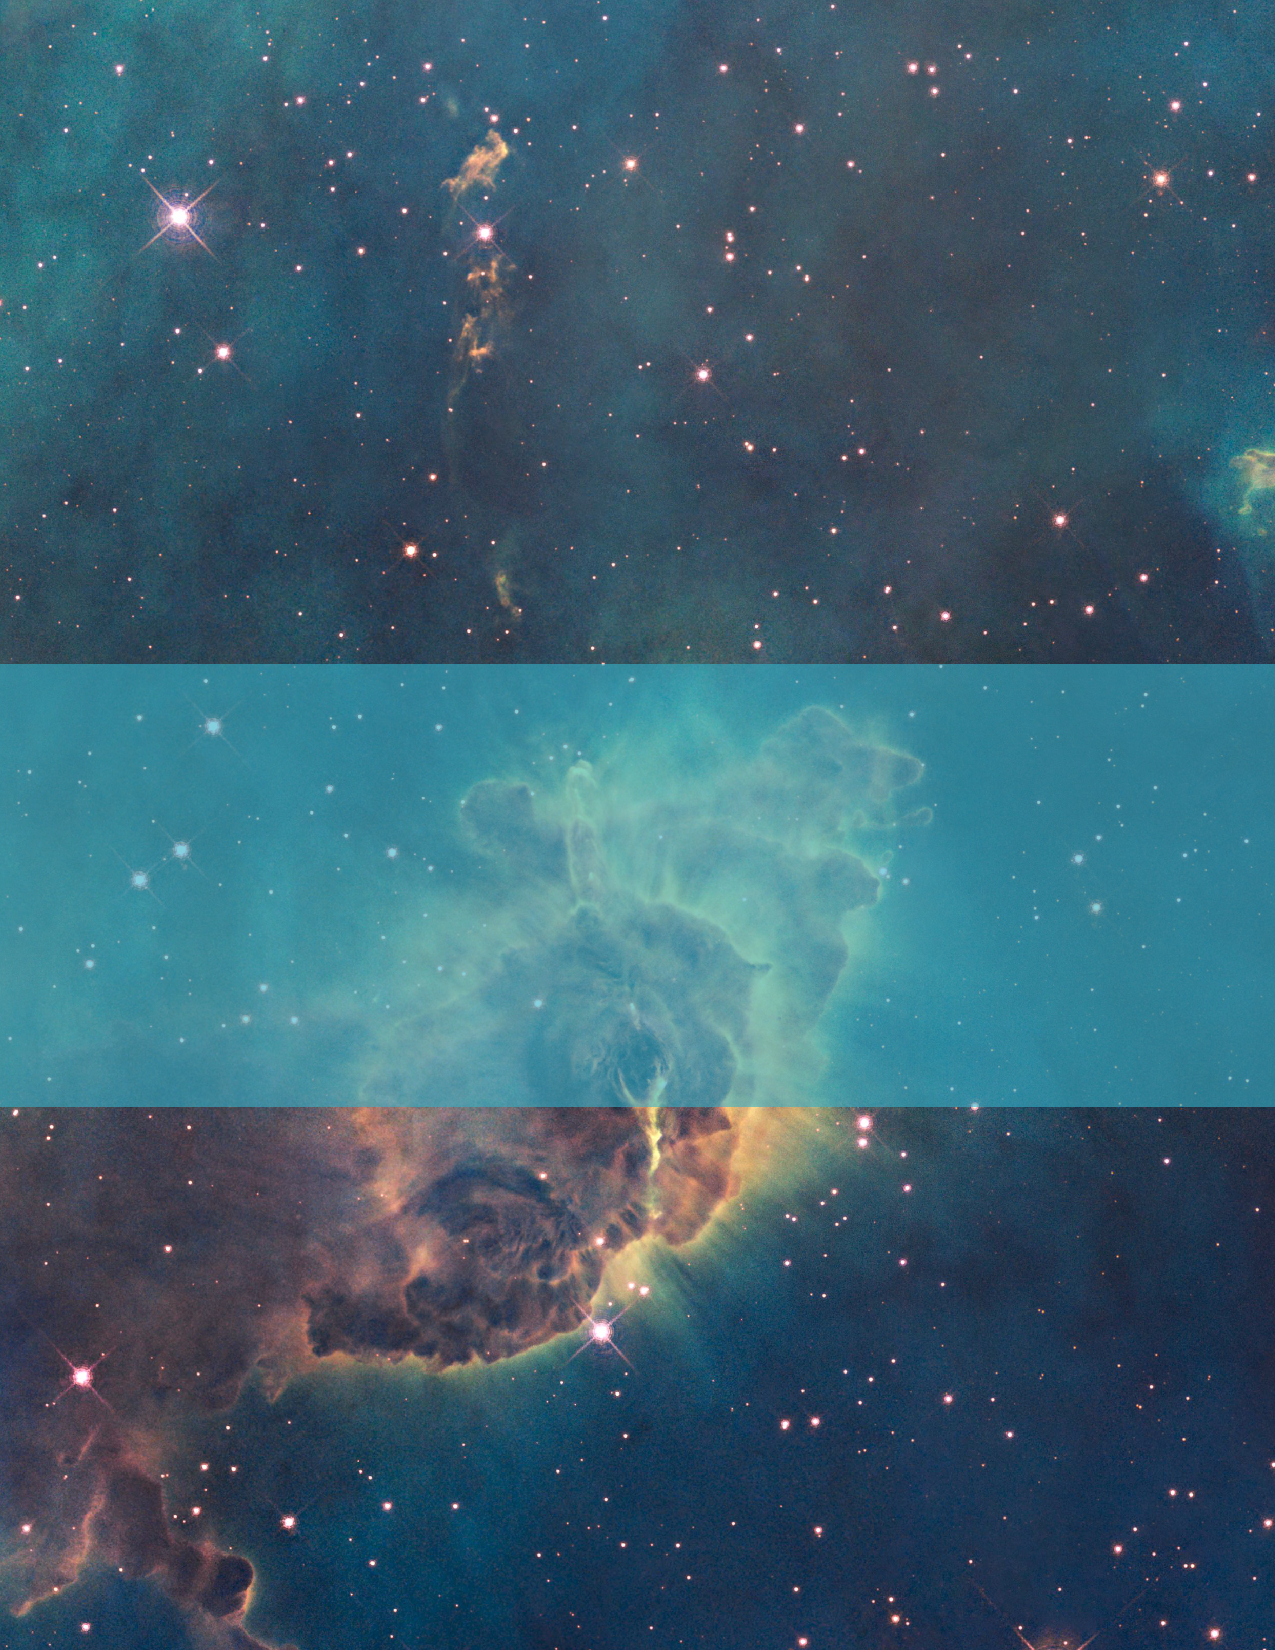
\includegraphics[scale=1.25]{esahubble}}} % Image background
\centering
\vspace*{5cm}
\par\normalfont\fontsize{35}{35}\sffamily\selectfont
\textbf{Algebra (Honor Track) Spring 2024}\\
\vspace*{0.4cm}
{\Huge \textbf{Communitative Algebra}}\par % Book title
\vspace*{0.4cm}
{\Huge Notes}\par % Author name
{\Large ymy}\par
\endgroup

%----------------------------------------------------------------------------------------
%	COPYRIGHT PAGE
%----------------------------------------------------------------------------------------

\newpage
~\vfill
\thispagestyle{empty}

%\noindent Copyright \copyright 2014 Andrea Hidalgo\\ % Copyright notice

\noindent \textsc{Personal use}\\

\noindent {https://github.com/flaricy/algebra-notes}\\ % URL

\noindent The author hopes to take notes while learning abstract algebra. Reference books are \textit{Introduction to communitative algebra} by \textit{Atiyah, Michael}. Starts from Feb 21st, 2024. 

%----------------------------------------------------------------------------------------
%	TABLE OF CONTENTS
%----------------------------------------------------------------------------------------

\chapterimage{head1.png} % Table of contents heading image

\pagestyle{empty} % No headers

\tableofcontents % Print the table of contents itself

%\cleardoublepage % Forces the first chapter to start on an odd page so it's on the right

\pagestyle{fancy} % Print headers again

\newpage
\thispagestyle{empty}
\centering 
\vspace*{10cm}
\textit{This page is intentionally left blank.}
%----------------------------------------------------------------------------------------
%	CHAPTER 1
%----------------------------------------------------------------------------------------

\chapterimage{head2.png} % Chapter heading image
\chapter{Group Theory}
\section{Groups and subgroups}
\begin{definition}
	[direct product] Let $(G, *)$ and $(H, \circ )$ be groups, then we may form a new group structure
	on $G \times H$ with group operation given by 
	\[(g, h) \star (g', h') = (g*g', h\circ h') \]
	This is called the {\bf direct product} of G and H.
\end{definition}

\subsection{Important Examples of Groups} 
\begin{definition}
	[Dihedral groups 二面体群] \[D_{2n} = \text{symmetric group of a reguler n-gon}\]
	It can be rewritten as 
	\[D_{2n} = \langle r,s | r^n = 1, s^2 = 1, rsr = s^{-1}\rangle \]
\end{definition}

\begin{definition}
	[Permutation Groups] Let $\Omega$ be a set. The set 
	\[S_\Omega = \{\text{bijections } \sigma: \Omega \xrightarrow{\thicksim} \Omega\}\]
	admits a group structure:
	\begin{itemize}
		\item the group operation is composition
		\item the identity element is $id$
		\item the inverse of the element $\sigma$ is the inverse map.
	\end{itemize}
	This $S_\Omega$ is called the symmetry group or the permutation group of $\Omega$.
	When $\Omega = \{1,2 ,...,n\}$, we write $S_n$ instead.
\end{definition}

\begin{definition}
	[cyclic groups] A group $H$ is called cyclic if it can be generated by one element $x$, i.e.
	\[H = \langle x\rangle \]	
\end{definition}

\begin{lemma}
	There are 2 kinds of cyclic groups up to isomorphism. \\
	(1) $H \cong \textbf{Z}_n$ \\
	(2) $H \cong \textbf{Z}$
\end{lemma}

\begin{definition}
	[The quaternion group] 
	\[Q_8 = \{1,-1,i,-i,j,-j,k,-k\}\]
\end{definition}

\section{cosets, Lagrange theorem, quotient groups}
\subsection{Conjugation, normal subgroups, and quotient groups.}
\begin{definition}
	[conjugate] Let $a, g \in G$, then $gag^{-1}$ is called the {\bf conjugate of $a$ by $g$}. 
\end{definition}
\begin{definition}
	[定义-命题] If $H$ is a subgroup of $G$ and $g \in G$, then $gHg^{-1}$
	:= $\{ghg^{-1}
	| h \in H\}$ is a
	subgroup, called the conjugate of H by g
\end{definition}
\begin{proof}
	We just need to verify that $\forall a,b \in H$, $gag^{-1}\cdot(gbg^{-1})^{-1} \in gHg^{-1}$. 
\end{proof}

\begin{definition}
	[normal subgroup] If $H \leq G$ and all conjugates of $H$ is $H$ itself, we denote $H \unlhd G$.
	Note that this condition is also equivalent to $gH = Hg$
	(as subsets) for any $g \in G$. 
\end{definition}

\begin{definition}
	[quotient group] Let $H \unlhd G$, then $\forall a,b \in G$, we define
	\[aH \cdot bH:=\{kl | k\in aH, l \in bH\} = abH\]
	as subsets of $G$. This defines a group structure on $G/H$, called the {\bf quotient group} or the {\bf factor group} of $G$ by $H$.  
\end{definition}

\subsection{Some Technical Results}
\begin{proposition}
	Let $H$ and $K$ be subgroups of a group $G$. Define $HK = \{hk | h\in H, k\in K\}$. When $G$ is finite, we have 
	\[|HK| = \frac {|H| \cdot |K|} {|H \cap K|}\]
\end{proposition}

\begin{proof}
	{\it to be written}
\end{proof}

The following lemmas tells when $HK$ is a (normal) subgroup.
\begin{lemma}
	Let $H$ and $K$ be subgroups of $G$. If $HK = KH$ as sets, then $HK$ is a subgroup of $G$.
	In particular, if $K$ is a normal subgroup, then $hK = Kh$ for any $h \in H$, and thus $HK = KH$ is a subgroup of $G$.
\end{lemma}
\begin{proof}
	We need to verify that $\forall h_1k_1 \cdot (h_2k_2)^{-1} = h_1k_1k_2^{-1}h_2^{-1}\in HK$. Since $h_1(k_1k_2^{-1}) \in HK = KH$, there exists $h,k$ such that $h_1k_1k_2^{-1} = kh$. 
	Then $khh_2^{-1} \in KH = HK$.
\end{proof}

\begin{lemma}
	If $H, K$ are both normal subgroups of $G$, then $HK$ is also a normal subgroup of $G$.
\end{lemma}
\begin{proof}
	$\forall g \in G$, we have $gHK = HgK = HKg$. 	
\end{proof}

\subsection{homomorphism}
\begin{definition}
	[Kernel as a group homomorphism] For a homomorphism $\phi: G \to H$ of groups, the {\bf kernel} is 
	\[ker \;\phi = \{g \in G | \phi(g) = e_H\}\]
\end{definition}

\begin{lemma}
	Let $\phi:G\to H$ be a group homomorphism. \\
	(1) The image $\phi(G)$ is a subgroup of $H$. \\
	(2) The kernel $ker \; \phi$ is a normal subgroup of $G$.
\end{lemma}
\begin{proof}
	(1) It follows from that $\phi(g_1)\phi(g_2)^{-1} = \phi(g_1g_2^{-1}) \in \phi(G)$ \\
	(2) If $g_1, g_2 \in ker \; \phi$, then 
	\[\phi(g_1g_2^{-1}) = e_He_H^{-1} = e_H\]
	For any $g' \in G$, and any $g \in ker \ \phi$, \[\phi(g'gg'^{-1}) = \phi(g')e_H\phi(g')^{-1} = e_H\]  
\end{proof}

\begin{lemma}
	A homomorphism $\phi: G \to H$ of groups is injective if and only if $ker \; \phi = \{e_G\}$.
\end{lemma}

\section{isomorphism theorems, composition series, statement of Holder Theorem}
\subsection{isomorphism theorems}

\begin{theorem}
	[The first isomorphism theorem] If $\phi: G \to H$ is a homomorphism of groups, then $ker \; \phi \unlhd G$ and \[
		G / ker \phi \cong \phi(G) \]
\end{theorem}

\begin{theorem}
	[The second homomorphism theorem] Let $G$ be a group, and let $A \leq G$ be a subgroup and $B \unlhd G$ a normal subgroup. Then $AB$ is a subgroup of G, $B \unlhd AB, A\cap B \unlhd A$, and 
	\[AB/B \cong A/(A\cap B)\]
\end{theorem}
\begin{proof}
	By lemma 1.2.2 we know $AB$ is a subgroup of $G$. \\
	For any $ab \in AB$, since $B$ is normal to $G$, $abB = aB = Ba$ and $aB = aBb = Bab$. So $B \unlhd AB$. \\
	It is clear that $A\cap B \leq A$. For any $a \in A, x \in A\cap B$, we have $axa^{-1} \in B$, since $B$ is normal. Also $axa^{-1} \in A$, since $x \in A$. So $A \cap B \unlhd A$. \\
	To show the isomorphism, we define $\phi: AB \to A/(A\cap B)$ by $\phi(ab) = a(A\cap B)$. It's easy to verify that $\phi$ is well-defined, surjective and a homomorphism, with $ker \phi = B$. By Theorem 1.3.1, we know the statement is true.
	\[\begin{tikzcd}
		AB && {A/(A\cap B)} \\
		\\
		& {AB/B}
		\arrow["\phi", two heads, from=1-1, to=1-3]
		\arrow["q"', from=1-1, to=3-2]
		\arrow["f"', from=3-2, to=1-3]
	\end{tikzcd}\]
\end{proof}

\begin{theorem}
	[The third isomorphism theorem] Let $G$ be a group and $H, K$ be normal subgroups with $H \leq K$. Then $K/H \unlhd G/H$, and 
	\[(G/H)/(K/H) \cong G/K\] 
\end{theorem}
\begin{proof}
	Consider the map 
	\[\begin{tikzcd}
		{\phi:} & {G/H} && {G/K} \\
		& gH && gK
		\arrow[from=1-2, to=1-4]
		\arrow[maps to, from=2-2, to=2-4]
	\end{tikzcd}\]
	\begin{itemize}
		\item $\phi$ is well-defined. We can simply redefine $\phi$ as $\phi(gH) = gH\cdot K = gK$ as product of subsets of $G$.
		\item $\phi$ is homomorphism. Easy to verify.
		\item $\phi$ is surjective.
		\item ker $\phi = \{gH | gK = K\} = \{gH | g \in K\} = K/H$. So $K/H \unlhd G/H$. And by the first isomorphism theorem, we statement holds.  
	\end{itemize}
\end{proof}

\begin{theorem}
	[The fourth isomorphism theorem/ Lattice isomorphism theorem] Let $G$ be a group and $N \unlhd G$. Then there is a bijection
	\[\begin{tikzcd}
		{\{subgroups \ of \ G \ containing \ N\}} && {\{subgroups \ of \ G/N\}} \\
		A && {A/N} \\
		{\pi^{-1}(\overline A)} && {\overline{A}}
		\arrow[tail reversed, from=1-1, to=1-3]
		\arrow[maps to, from=2-1, to=2-3]
		\arrow[maps to, from=3-3, to=3-1]
	\end{tikzcd}\]
	where $\pi: G \to G/N$ is the natural projection. \\
	This bijection preserves
	\begin{itemize}
		\item inclusion of groups 
		\item intersections
		\item normality of subgroups 
		\item quotients of subgroups 
	\end{itemize}
	Visually, we have: Lattice of subgroups of G containing N $\iff$ Lattice of subgroups of G/N. 
\end{theorem}

\section{Lattice}
\begin{definition}
	Let (S, $\leq$) be a set equipped with a partial order. (S, $\leq$) is called a {\it Lattice} if any $x, y \in S, \{x, y\}$ has a maximal lower bound and a minimal upper bound.  
	The lower bound is denoted by $x \wedge y$, while the upper bound is denoted by $x \vee y$.
\end{definition}

\begin{example}
	设 n 为正整数,$A_n$ 为 n 的所有正因数的几何,则 $A_n$ 关于整除关系构成格。
\end{example}
\begin{example}
	设 $P(B)$ 为 $B$ 的幂集,则 $P(B)$ 关于包含关系 $\subseteq$ 构成格,称为幂集格.
\end{example}

\begin{example}
	[子群格] 群G的所有子群,关于包含关系。
\end{example}

\section{composition series, Jordan-Holder Theorem, simplicity of An, direct product groups}
\begin{definition}
	[composition series] In a group $G$, a series of subgroups 
	\[\{0\} = N_0 \leq N_1 \leq ... \leq N_k = G\]	
	such that $N_{i-1} \unlhd N_i$ and $N_i / N_{i-1}$ is a simple group for $1 \leq i \leq k$ is called {\bf composition series}. In this case, $N_i / N_{i-1}$ is called a {\bf composition factor}.
\end{definition}

\begin{definition}
	[solvable] A group G is called {\bf solvable} if there exists a composition series 
	\[\{0\} = N_0 \leq N_1 \leq ... \leq N_k = G\] 
	such that $N_i / N_{i-1}$ is abelian.
\end{definition}

\begin{corollary}
	a finite group is solvable if and only if all the composition factors are $\mathbf{Z}_p$.
\end{corollary}

\begin{theorem}
	[Jordan-Holder] Let G be a non-trivial group, \\ 
	(1) G has a composition series. \\(2) Assume that a group $G$ has the following two composition series, 
	\[\{0\} = A_0 \leq A_1 \leq ... \leq A_m = G, \quad \{0\} = B_0 \leq B_1 \leq ... \leq B_n = G\]
	then $m = n$ and there exists a bijection $\sigma:\{1,2,...,m\}\to \{1,2,...,n\}$
	\[A_{\sigma(i)} / A_{\sigma(i-1)} \cong B_i / B_{i-1}\]
	for $i = 1, 2, ... m$
\end{theorem}

\begin{proof}
	{\it to be written}
\end{proof}

\subsection{The simplicity of An, n >= 5}

\begin{proposition}
	
\end{proposition}
%%% -------------------------
%%%  chapter{Rings and Ideals}
%%%
\chapterimage{destiny2_resized.jpg} % Chapter heading image
\chapter{Rings and Ideals}
If not pointed out specifically, the notion "ring" refers to a commutative ring with an identity element. 

\section{rings, ideals, quotient rings}
\begin{definition}
	[ring homomorphism] Let $A, B$ be rings, $f : A\to B$ is a homomorphism when \\
	(1) $f(x+y) = f(x) + f(y)$. So $f$ is a homomorphism of abelian groups. \\
	(2) $f(xy) = f(x)f(y)$, $f(1) = 1$. So $f$ is a homomorphism between the monoids $(A, \cdot)$ and $(B, \cdot)$.

\end{definition}
\begin{definition}
	[ideal of a ring] An ideal $I$ of a ring $A$ is an additive subgroup and is such that $A\I \subseteq I$.
\end{definition}
\begin{example}
	Every ring $A$ has 2 trivial ideals: $\{0\}$ and $A$.
\end{example}

Below, $I$ denotes the ideal of ring $A$.
\begin{definition}
	[quotient ring] Define multiplication in the quotient group $A/\I$ by\\
	\[(a + I) \cdot (b + I) = ab + I\]
	It is well defined. Now $A/I$ is made into a ring called the {\it quotient ring}. The mapping $\phi: A \to A/I$ which maps each $x \in A$ to its coset $x + I$ is a surjective ring homomorphism.
\end{definition}

\begin{proposition}
	There is a one-to-one order preserving correspondence between 
	\[\begin{tikzcd}
		{\{J|I\subseteq J \subseteq A, J:ideal\}} && {\{\overline{J} | ideal \; \overline{J} \subseteq A/I\}} \\
		J && {J + I} \\
		{\phi^{-1}(\overline{J})} && {\overline{J}}
		\arrow["{1:1}", tail reversed, from=1-1, to=1-3]
		\arrow[maps to, from=2-1, to=2-3]
		\arrow[maps to, from=3-3, to=3-1]
	\end{tikzcd}\]
\end{proposition}
\begin{proof}
	First, Let's show that $J + I$ is an ideal in $A/I$. \\
	$J + I$ is abelian : trivial; $\forall x + I \in A/I, (x+I)\cdot(J+I) = (Jx + I) \subseteq (J+I) $, since $J$ is an ideal. \\
	Second, we can verify this mapping to be invertible.

\end{proof}

\begin{corollary}
	If $f: A\to B$ is any ring homomorphism, the {\it kernel} of $f(=f^{-1}(0))$ is an ideal of $A$, and the image of $f (= f(A))$ is a subring $C$ of $B$, but may not be an ideal.
\end{corollary}
\begin{proof}
	Consider the embedding mapping\[\begin{tikzcd}
		{\mathbb{Q} } && {\mathbb{Q}[X]}
		\arrow[hook, from=1-1, to=1-3]
	\end{tikzcd}\]
	The image is absolutely not an ideal.
\end{proof}

\begin{theorem}
	[fundamental homomorphism theorem] $f: A \to B$ is a ring homomorphism, $I$ is the kernel of $f$, $g(a + I) := f(a)$ then $g$ is a ring isomorphism.
	\[\begin{tikzcd}
		A && {Im(f)} && B \\
		\\
		&& {A/I}
		\arrow["f", two heads, from=1-1, to=1-3]
		\arrow[hook, from=1-3, to=1-5]
		\arrow["g", from=3-3, to=1-3]
		\arrow["\phi", from=1-1, to=3-3]
	\end{tikzcd}\]

\end{theorem}

\section{zero-divisors, nilpotent elements, units}
\begin{definition}
	[zero-divisor] a zero-divisor in a ring $A$ is an element $x$ for which there exists $y \neq 0$ in $A$ such that $xy = 0$
\end{definition}
\begin{definition}
	[integral domain] a ring with no zero-divisors $\neq 0$ and not a zero ring.
\end{definition}

\begin{definition}
	[nilpotent] An element $x \in A$ is {\it nilpotent} if $x^n = 0$ for some $n > 0$.
\end{definition}
\begin{remark}
	A nilpotent element is a zero-divisor.
\end{remark}

\begin{definition}
	[unit 可逆元] A unit in $A$ is an element $x$ such that $xy = 1$ for some $y \in A$. Note that $y$ is uniquely determined by $x$, and is written as $x^{-1}$. 
\end{definition}
\begin{remark}
	The units in $A$ form a abelian group under multiplication.
\end{remark}

\begin{definition}
	[field] A field is a ring $A$ which $1 \neq 0$ and every non-zero elem. is a unit.
\end{definition}

\begin{proposition}
Let A be a ring $\neq 0$. The following are equivalent:\\
(1) A is a field;\\
(2) The only ideals in A are ${0}$ and $(1)$; \\
(3) Every non-trivial homomorphism of A into a non-zero ring B is injective.	
\end{proposition}

\section{prime ideals and maximal ideals}
\newcommand{\fp}{\mathfrak{p}}
\newcommand{\fm}{$\mathfrak{m}$}
\begin{definition}
	[prime ideal]An ideal $\fp$ in $A$ is {\it prime} if $\fp \neq (1)$ and if $xy \in \fp \implies x\in \fp$ or $y \in \mathfrak{p}$ 
\end{definition}

\begin{definition}
	[maximal ideal] An ideal \fm in $A$ is {\it maximal} if \fm $\neq (1)$ and if there is no ideal $\alpha $ such that \fm $\subset \alpha \subset (1)$(strict inclusion).
\end{definition}
\begin{remark}
	\fm \text{ can} be $\{0\}$.
\end{remark}

\begin{proposition}
	$\fp$ is prime $\iff$ $A/\fp$ is an integral domain.
\end{proposition}
\begin{proof}
	Easy to verify.
\end{proof}

\begin{proposition}
	\fm \text{ }is maximal $\iff$ $A/m$ is a field. Hence, a maximal ideal is prime.
\end{proposition}
\begin{proof}
	By Proposition 2.1.1 and Proposition 2.2.1, the statement holds.
\end{proof}

\begin{proposition}
	If $f: A\to B$ is a ring homomorphism and $q$ is a prime ideal of $B$, then $f^{-1}(q)$ is a prime ideal in $A$.
\end{proposition}
\begin{proof}
	If $a, b \in A$ such that $f(a) = f(b) \in q$. Then $f(a-b) = f(a)-f(b) \in q$. Thus, $f^{-1}(q)$ is abelian. For any $a \in f^{-1}(q), x \in A$, we have 
	$f(ax) = f(a)f(x) \in Bq = q$. Thus, $f^{-1}(q)$ is an ideal. For any $a, b\in A, ab \in f^{-1}(q) \iff f(ab) \in q \iff f(a)\cdot f(b)\in q \iff f(a) \in q \vee f(b) \in q \iff a \in f^{-1}(q) \vee b \in f^{-1}(q) \iff f^{-1}(q)$ is a prime ideal.  	
\end{proof}

\begin{remark}
	If $m$ is a maximal ideal of $B$, it is not necessarily true that $f^{-1}(m)$ is maximal in $A$. Consider $A = \mathbb{Z}, B = \mathbb{Q}, m = \{0\}$.
\end{remark}

\begin{theorem}
	Every ring $A \neq 0$ has at least one maximal ideal.
\end{theorem}
This theorem relys on Zorn's Lemma. We first introduce it.

\begin{definition}
	[chain in a partially ordered set] Let $S$ be a non-empty partially ordered set. A subset $T$ of $S$ is a chain if either $x \leq y$ or $y \leq x$ for every pair of elements in $T$.
\end{definition}

\begin{lemma}
	[Zorn] If every chain $T$ of $S$ has an upper bound in $S$, then $S$ has at least one maximal element. Zorn's Lemma is equivalent to the axiom of choice.
\end{lemma}

\begin{proof}
	Let's prove theorem 2.3.4, using Zorn's Lemma. \\
	Let $\Sigma = \{I : I \ is \ ideal, I \neq (1)\}$. Order $\Sigma$ by inclusion. $\Sigma$ is not empty, since $0 \in \Sigma$. For each chain, consider the union as another ideal $\neq (1)$ to be an upper bound. Then Zorn's lemma yields that there is a maximal element.
\end{proof}
\begin{remark}
	If $A$ is Noetherian, we can avoid the use of Zorn's lemma.	
\end{remark}

\begin{corollary}
	If $a \neq (1)$ is an ideal of $A$, there exists a maximal ideal of $A$ containing $a$.
\end{corollary}
\begin{proof}
	Replace $\Sigma$ by $\{I: I \ is \ ideal \ containing \ a, I \neq (1)\}$ in the proof of Theorem 2.3.4 .
\end{proof}

\begin{corollary}
	Every non-unit of $A$ is contained in a maximal ideal.
\end{corollary}

\begin{definition}
	[local ring, residue field] If a ring $A$ has exactly one maximal ideal $m$ (e.g. fields), then $A$ is called a {\it local ring}. The field $k = A/m$ is called the residue field of $A$.
\end{definition}

\begin{proposition}
	Let $A$ be a ring and $m \neq (1)$ an ideal of $A$ such that $\forall x \in A - m$ is a unit in $A$. Then $A$ is a local ring and $m$ its maximal ideal.
\end{proposition}

First, we observe the following
\begin{lemma}
	Every element in a maximal ideal is not a unit.
\end{lemma}

\begin{proof}[proof of Proposition 2.3.8]
	From corollary 2.3.6 and lemma 2.3.9 we know $m$ is a maximal ideal. Also from lemma 2.3.9, we know there doesn't exists other maximal ideals. Thus, $A$ is a local ring.
\end{proof}

\begin{proposition}
	Let $A$ be a ring and $m$ a maximal ideal, such that every element of $1 + m$ is a unit in $A$. Then $A$ is a local ring.
\end{proposition}
\begin{proof}
	Make an analogy to Bezout Theorem. Let $x \in A - m$. Since $m$ is maximal, the ideal generated by $x$ and $m$ is $(1)$, hence there exists $y \in A, t\in m$ such that $xy + t = 1$.
	Thus $xy = 1 - t \in 1 + m$, which means $x$ is a unit. 
\end{proof}

\begin{example}
	$A = F[X_1,...,X_n], F$ : field. Let $f \in A$ be an irreducible polynomial. By unique factorization, the ideal $(f)$ is prime. When $n \geq 2$, it's not a {\it principal ideal domain}.	
\end{example}

\begin{example}
	Every ideal in $\mathbf{Z}$ is of the form $(m)$ for some $m \geq 0$. The ideal is prime $\iff$ $m = 0$ or is a prime number. For all ideals $(p)$ are maximal.
\end{example}

\begin{definition}
	[principal integral domain] an integral domain where every ideal is principal.
\end{definition}

\begin{proposition}
	Every non-zero prime ideal is maximal.
\end{proposition}
\begin{proof}
	[Hint] The cancellation law applies in the integral domain.
\end{proof}

\section{nilradical and Jacobson radical}
\begin{proposition}
	The set $\mathfrak{R}$ of all nilpotent elements in a ring $A$ is an ideal, and $A / \mathfrak{R}$ has no nilpotent element $\neq 0$.
\end{proposition}
\begin{proof}
	For any $x,y \in \mathfrak{R}$, there exists $n \geq 0$ such that, $(x-y)^n = 0$. Thus, $x - y \in \mathfrak{R}$ and $\mathfrak{R}$ is abelian group. It's easy to show that $\mathfrak{R}$ is an ideal.
	If there exists $a \in A$, such that $\exists n > 0, (a + \mathfrak{R})^n = 0 = a^n + \mathfrak{R}$ , then $a \in \mathfrak{R}$. Hence, $A / \mathfrak{R}$ has no non-zero nilpotent element.
\end{proof}

The ideal $\mathfrak{R}$ is called the {\it nilradical} of $A$.
\begin{proposition}
	The nilradical of $A$ is the intersection of all the prime ideals of $A$.
\end{proposition}
\begin{proof}
	We observe that every nilpotent element belongs to any prime ideal. Hence, $\mathfrak{R} \subseteq \cap_{p:prime \ ideal}p$.
	On the other side, for each element within the intersection of all prime ideals, 试图用Zorn's lemma寻找一个极大理想,证明这也是一个prime ideal. 从而non-nilpotent element不属于这个ideal.
\end{proof}

\begin{definition}
	[Jacobson radical] The Jacobson radical $\mathfrak{R}$ of $A$ is defined to be the intersection of all the maximal ideals of $A$.
\end{definition}
It can be characterized as
\begin{proposition}
	$x\in \mathfrak{R} \iff 1 - xy$ is a unit for all $y \in A$.
\end{proposition}
\begin{proof}
	$\implies$: Suppose $1-xy$ is not a unit. By corollary 2.3.7 it belongs to some maximal ideal $m$. But $x\in \mathfrak{R}\subseteq m$, hence $xy \in m$ and $1 \in m$, which is absurd. \\
	$\Leftarrow$: 考虑Bezout定理。If $x\notin m$ for some maximal ideal $m$, then $m + (x)$ generate the unit ideal $(1)$, so that $u + xy = 1$ for some $u \in m, y \in A$. Hence $1 - xy \in m$ is not a unit.
\end{proof}

\section{operations on ideals}

\chapterimage{town_resized.png} % Chapter heading image
\chapter{Module Theory}

% file ending
\end{CJK}
\end{document}
